\documentclass{standalone}
\usepackage{tikz}
\begin{document}
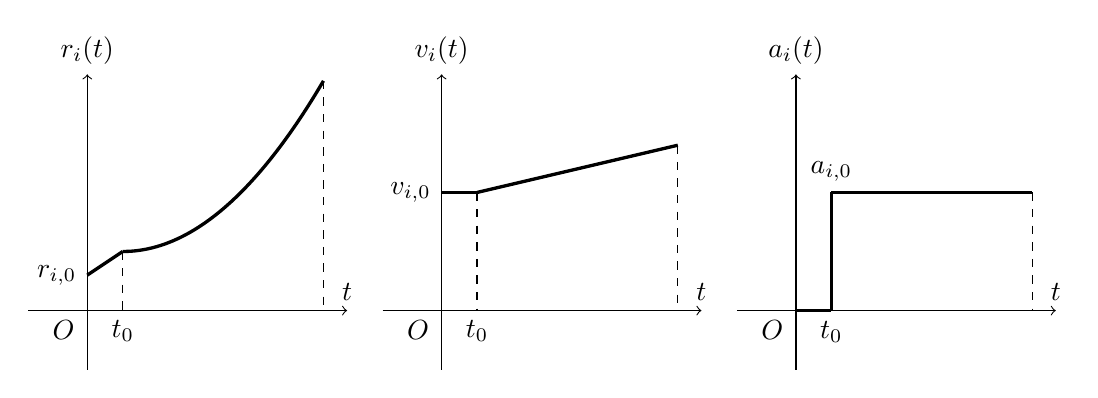
\begin{tikzpicture}[scale = 1.5]
    \coordinate (O) at (-3,0);
    \node[below] at (-3.2,0) {$O$};
    \draw[->] (-3.5, 0) -- (-0.8, 0) coordinate (t) node[above]{$t$};
    \draw[->] (-3,-0.5) --(-3,2) coordinate (s) node[above]{$r_i(t)$};
    \draw[-,very thick] (-3, 0.3) node[left] {$r_{i,0}$} -- (-2.7,0.5);
    \draw[dashed] (-2.7, 0.5) -- (-2.7, 0) node[below] {$t_0$};
    \draw[very thick] plot[smooth, domain=-2.7:-1](\x,{0.5+0.5*(\x+2.7)^2});
    \draw[dashed] (-1,1.945) -- (-1, 0);


    \coordinate (O) at (0,0);
    \node[below] at (-0.2,0) {$O$};
    \draw[->] (-0.5, 0) -- (2.2, 0) coordinate (t) node[above]{$t$};
    \draw[->] (0,-0.5) --(0,2) coordinate (s) node[above]{$v_i(t)$};
    \draw[-,very thick] (0, 1)  node[left] {$v_{i,0}$} -- (0.3, 1);
    \draw[dashed] (0.3, 1) -- (0.3, 0) node[below] {$t_0$};
    \draw[-,very thick] (0.3, 1) -- (2,1.4);
    \draw[dashed] (2,1.4) -- (2, 0);


    \coordinate (O) at (3,0);
    \node[below] at (2.8, 0) {$O$};
    \draw[->] (2.5, 0) -- (5.2, 0) coordinate (t) node[above]{$t$};
    \draw[->] (3,-0.5) --(3,2) coordinate (v) node[above]{$a_i(t)$};
    \draw[very thick](3,0)--(3.3,0);
    \draw[-,very thick] (3.3, 1)node[above] {$a_{i,0}$} -- (3.3, 0) node[below] {$t_0$};
    \draw[-,very thick] (3.3, 1) -- (5,1);
    \draw[dashed] (5,1) -- (5, 0);
\end{tikzpicture}
\end{document}